\part{Entrega 1}
Claro, aquí tienes el texto corregido:

\section{Introducción}
Las estructuras que se utilizan en el espacio deben contar con una serie de características que les permitan operar y cumplir con su función de forma eficiente y segura. Una de estas características es la relación de masa estructural y la longitud de la estructura con las frecuencias y modos de vibración de la misma. Si estos requisitos no se cumplen, mandar la estructura al espacio además de ser costoso, puede ser peligroso para la tripulación y la misión.

En este informe se estudiarán varias relaciones de masa estructural para obtener un área óptima de un reticulado, junto con la determinación de los modos de vibración que sean mayores a 0.1 Hz, ya que esta es una frecuencia que se considera segura en el espacio.

Para cumplir con este objetivo, se emplearán la librería OpenSeesPy para el análisis estructural y la identificación de las frecuencias y modos de vibración de la estructura, y PyVista para la visualización de los datos obtenidos.
\newpage
\section{Modelo}


\section{Resultados}

\subsection{Caso de 2 vanos}
En el caso de 2 vanos se obtuvieron los siguientes diametros de las barras de fibra de carbono, además, se muestran los porcentajes de RME.

\begin{table}[H]
    \centering
    \begin{tabular}{cccc}
    \toprule
     A & Diametro exterior [mm] & Diametro interior [mm] & RME [\%] \\
    \midrule
     $A_{10\%}$ &  4 &  2.6 &  10.89 \\
     $A_{20\%}$ &  5 &  2.5 &  22.11 \\
     $A_{30\%}$ &  5.8 &  2.4 &  32.88 \\
    \bottomrule
    \end{tabular}
\end{table}

Donde se obtuvieron las siguientes frecuencias de vibración para cada porcentaje de RME.

\begin{table}[H]
    \centering
    \begin{tabular}{cccc}
    \toprule
     Frecuencia (Hz) & $A_{10\%}$ & $A_{20\%}$ & $A_{30\%}$ \\
    \midrule
     1 &  0.245 &  0.349 &  0.425 \\
     2 &  0.283 &  0.400 &  0.484 \\
     3 &  0.314 &  0.445 &  0.540 \\
     4 &  0.666 &  0.947 &  1.154 \\
     5 &  0.673 &  0.958 &  1.166 \\
     6 &  0.744 &  1.054 &  1.280 \\
     7 &  1.014 &  1.442 &  1.757 \\
     8 &  1.046 &  1.488 &  1.812 \\
     9 &  1.206 &  1.717 &  2.092 \\
     10 &  1.454 &  2.070 &  2.522 \\
    \bottomrule
    \end{tabular}
\end{table}

En este caso todas las combinaciones logran la frecuencia fundamental esperada, ya que en todos los casos es mayor a 0.1 Hz, además, se puede observar que a medida que aumenta el porcentaje de RME, las frecuencias también aumentan.

A continuacion se muestra un grafico de la frecuencia para cada modo de vibración y cada RME. 

\begin{figure}[H]
    \centering
    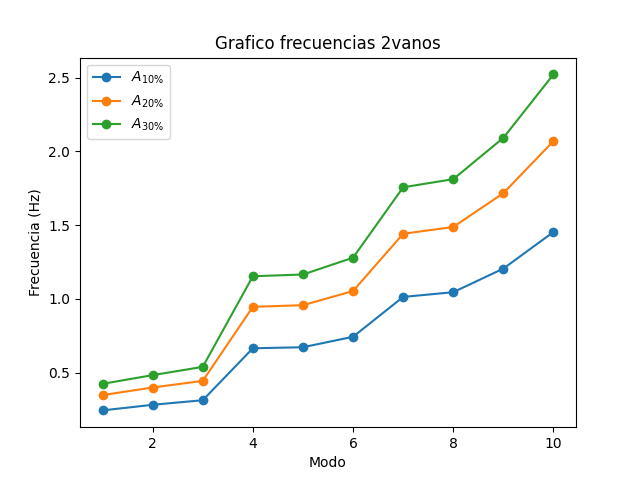
\includegraphics[width=0.8\textwidth]{../grafico_frecuencias_2vanos.png}
    \caption{Frecuencia de vibración para cada modo de vibración y cada RME.}
\end{figure}

\subsection{Caso de 4 vanos}
En el caso de 4 vanos se obtuvieron los siguientes diametros de las barras de fibra de carbono, además, se muestran los porcentajes de RME.

\begin{table}[H]
    \centering
    \begin{tabular}{cccc}
    \toprule
     A & Diametro exterior [mm] & Diametro interior [mm] & RME [\%] \\
    \midrule
     $A_{10\%}$ &  4 &  2.6 &  10.41 \\
     $A_{20\%}$ &  5 &  2.5 &  21.13 \\
     $A_{30\%}$ &  5.8 &  2.4 &  31.41 \\
    \bottomrule
    \end{tabular}
\end{table}

Donde se obtuvieron las siguientes frecuencias de vibración para cada porcentaje de RME.

\begin{table}[H]
    \centering
    \begin{tabular}{cccc}
    \toprule
     Frecuencia (Hz) & $A_{10\%}$ & $A_{20\%}$ & $A_{30\%}$ \\
    \midrule
     1 &       0.103 &       0.146 &       0.175 \\
     2 &       0.141 &       0.195 &       0.228 \\
     3 &       0.162 &       0.228 &       0.272 \\
     4 &       0.342 &       0.486 &       0.582 \\
     5 &       0.393 &       0.553 &       0.656 \\
     6 &       0.449 &       0.633 &       0.754 \\
     7 &       0.597 &       0.849 &       1.015 \\
     8 &       0.624 &       0.887 &       1.060 \\
     9 &       0.688 &       0.974 &       1.162 \\
     10 &       0.735 &       1.039 &       1.236 \\
    \bottomrule
    \end{tabular}
\end{table}

En este caso se puede observar que todas las combinaciones logran la frecuencia esperada, ya que todas son mayores a 0.1 Hz.

A continuacion se muestra un grafico de la frecuencia para cada modo de vibración y cada RME. 

\begin{figure}[H]
    \centering
    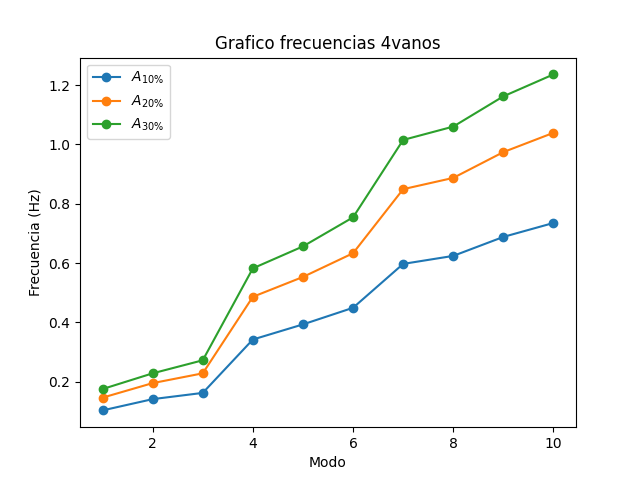
\includegraphics[width=0.8\textwidth]{../grafico_frecuencias_4vanos.png}
    \caption{Frecuencia de vibración para cada modo de vibración y cada RME.}
\end{figure}

\subsection{Caso de 8 vanos}
En el caso de 8 vanos se obtuvieron los siguientes diametros de las barras de fibra de carbono, además, se muestran los porcentajes de RME.

\begin{table}[H]
    \centering
    \begin{tabular}{cccc}
    \toprule
     A & Diametro exterior [mm] & Diametro interior [mm] & RME [\%] \\
    \midrule
     $A_{10\%}$ &  4 &  2.6 &  10.17 \\
     $A_{20\%}$ &  5 &  2.5 &  20.63 \\
     $A_{30\%}$ &  5.8 &  2.4 &  30.68 \\
    \bottomrule
    \end{tabular}
\end{table}

Donde se obtuvieron las siguientes frecuencias de vibración para cada porcentaje de RME.

\begin{table}[H]
    \centering
    \begin{tabular}{cccc}
    \toprule
     Frecuencia (Hz) & $A_{10\%}$ & $A_{20\%}$ & $A_{30\%}$ \\
    \midrule
     1 &       0.035 &       0.049 &       0.059 \\
     2 &       0.064 &       0.083 &       0.095 \\
     3 &       0.081 &       0.115 &       0.139 \\
     4 &       0.147 &       0.208 &       0.253 \\
     5 &       0.195 &       0.266 &       0.314 \\
     6 &       0.234 &       0.330 &       0.399 \\
     7 &       0.307 &       0.435 &       0.528 \\
     8 &       0.336 &       0.474 &       0.574 \\
     9 &       0.388 &       0.548 &       0.663 \\
     10 &       0.444 &       0.629 &       0.760 \\
    \bottomrule
    \end{tabular}
\end{table}

En este caso se puede observar que ninguna de las combinaciones logra la frecuencia fundamental esperada, ya que en todos los casos es menos a 0.1 Hz.

A continuacion se muestra un grafico de la frecuencia para cada modo de vibración y cada RME. 

\begin{figure}[H]
    \centering
    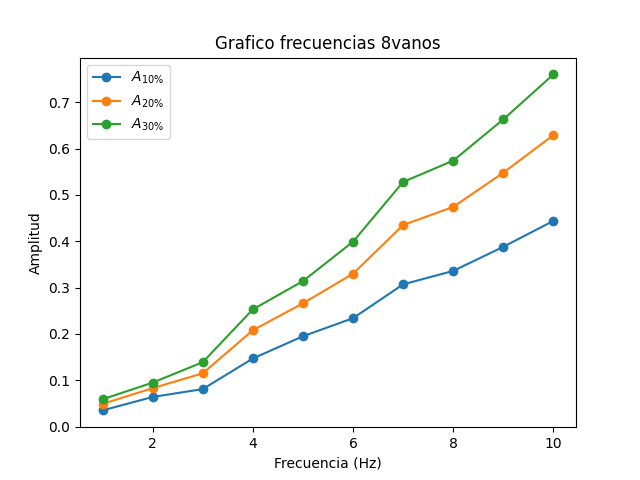
\includegraphics[width=0.8\textwidth]{../grafico_frecuencias_8vanos.png}
    \caption{Frecuencia de vibración para cada modo de vibración y cada RME.}
\end{figure}

\subsection{Caso de 16 vanos}
En el caso de 16 vanos se obtuvieron los siguientes diametros de las barras de fibra de carbono, además, se muestran los porcentajes de RME.

\begin{table}[H]
    \centering
    \begin{tabular}{cccc}
    \toprule
     A & Diametro exterior [mm] & Diametro interior [mm] & RME [\%] \\
    \midrule
     $A_{10\%}$ &  4 &  2.6 &  10.05 \\
     $A_{20\%}$ &  5 &  2.5 &  20.39 \\
     $A_{30\%}$ &  5.8 &  2.4 &  30.32 \\
    \bottomrule
    \end{tabular}
\end{table}

Donde se obtuvieron las siguientes frecuencias de vibración para cada porcentaje de RME.

\begin{table}[H]
    \centering
    \begin{tabular}{cccc}
    \toprule
     Frecuencia (Hz) & $A_{10\%}$ & $A_{20\%}$ & $A_{30\%}$ \\
    \midrule
     1 &       0.010 &       0.014 &       0.017 \\
     2 &       0.025 &       0.029 &       0.031 \\
     3 &       0.040 &       0.057 &       0.069 \\
     4 &       0.052 &       0.074 &       0.090 \\
     5 &       0.086 &       0.112 &       0.130 \\
     6 &       0.113 &       0.160 &       0.194 \\
     7 &       0.130 &       0.184 &       0.223 \\
     8 &       0.161 &       0.222 &       0.264 \\
     9 &       0.192 &       0.270 &       0.326 \\
     10 &       0.212 &       0.299 &       0.363 \\
    \bottomrule
    \end{tabular}
\end{table}

En este caso se puede observar que ninguna de las combinaciones logra la frecuencia fundamental esperada, ya que en todos los casos es menos a 0.1 Hz.

A continuacion se muestra un grafico de la frecuencia para cada modo de vibración y cada RME. 

\begin{figure}[H]
    \centering
    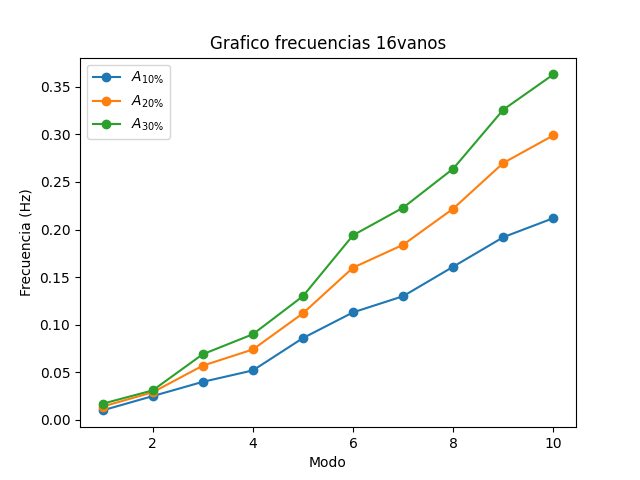
\includegraphics[width=0.8\textwidth]{../grafico_frecuencias_16vanos.png}
    \caption{Frecuencia de vibración para cada modo de vibración y cada RME.}
\end{figure}

\subsection{Comparación de los casos}

En este caso se puede observar que a medida que aumenta el número de vanos, las frecuencias de vibración disminuyen, además, se puede observar que a medida que aumenta el porcentaje de RME, las frecuencias también aumentan. Por lo que se puede decir que la estructura con mayor frecuencia es la del caso de 2 vanos con un porcentaje de RME del 30\%, y la con menor frecuencia es la del caso de 16 vanos con un porcentaje de RME del 10\%.\\
Además, se puede observar que no en todos los casos se logro la frecuencia fundamental minima esperada de 0.1 Hz. En este caso, los que lograron la frecuencia fundamental minima esperada fueron los casos de 2 y 4 vanos, mientras que los casos de 8 y 16 vanos no lograron la frecuencia fundamental minima esperada.

\section{Conclusiones}